\begin{center}
    \textbf{Geração 1000}
\end{center}

\begin{figure}[h]
    \centering
    \label{fig:geracao01}
    
    \begin{tabular}{rl}
        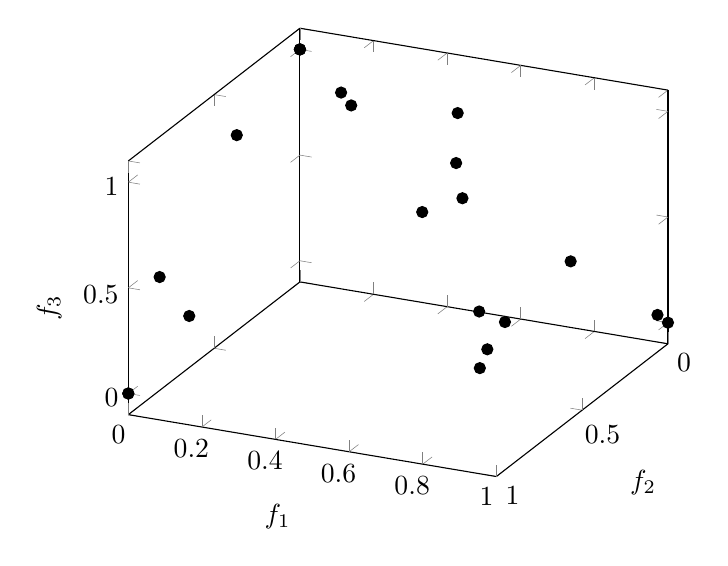
\begin{tikzpicture}[scale=1.0]
        	\begin{axis}[xlabel=$f_2$, ylabel=$f_1$, zlabel=$f_3$, view/h=115]
    			\addplot3[only marks] coordinates {
            		(1.000000, 0.000000, 0.000000) (1.000000, 0.000000, 0.000000) (0.000000, 1.000000, 0.000000) (0.000000, 0.000000, 1.000000) (0.000000, 0.000000, 1.000000) (0.000000, 0.000000, 1.000358) (0.363503, 0.611054, 0.703192) (0.076016, 0.464061, 0.882536) (0.274681, 0.863668, 0.422643) (0.567388, 0.751617, 0.336368) (0.471063, 0.551938, 0.688087) (0.591789, 0.785122, 0.182675) (0.267845, 0.549297, 0.791538) (0.619282, 0.777599, 0.108764) (0.220880, 0.242300, 0.944724) (0.876126, 0.027342, 0.481306) (0.177735, 0.194732, 0.964619) (0.527656, 0.803138, 0.276690) (0.924683, 0.130411, 0.357706) (0.453043, 0.039654, 0.890606) (0.052963, 0.996228, 0.068737) 

        		};
        	\end{axis}
	    \end{tikzpicture}
	    &
	    \begin{tikzpicture}[scale=1.0]
        	\begin{axis}[xlabel=$f_2$, ylabel=$f_1$, zlabel=$f_3$, view={45}{0}]
    			\addplot3[only marks] coordinates {
            		(1.000322,0.000000,0.000000)(0.000000,1.000322,0.000000)(0.000000,0.000000,1.000322)(0.000000,0.000000,1.000322)(0.000000,0.000000,1.002923)(0.955769,0.258176,0.143162)(0.691769,0.330831,0.642382)(0.593392,0.615999,0.518725)(0.177695,0.120517,0.977013)(0.275671,0.566808,0.776775)(0.020085,0.895169,0.445999)(0.858969,0.451363,0.243083)(0.249082,0.540673,0.803914)(0.056891,0.491929,0.869201)(0.007708,0.699945,0.714606)(0.037079,0.195407,0.980394)(0.759974,0.421622,0.495376)(0.421243,0.394921,0.816898)(0.000000,0.927199,0.375431)(0.510850,0.007446,0.860013)(0.102136,0.797748,0.594885) 

        		};
        	\end{axis}
	    \end{tikzpicture}
	\end{tabular}
    
\end{figure}

